% !TEX root = ../main.tex



\subsection{Plaatsvector}

\begin{frame}{Plaatsvector}
\begin{figure}
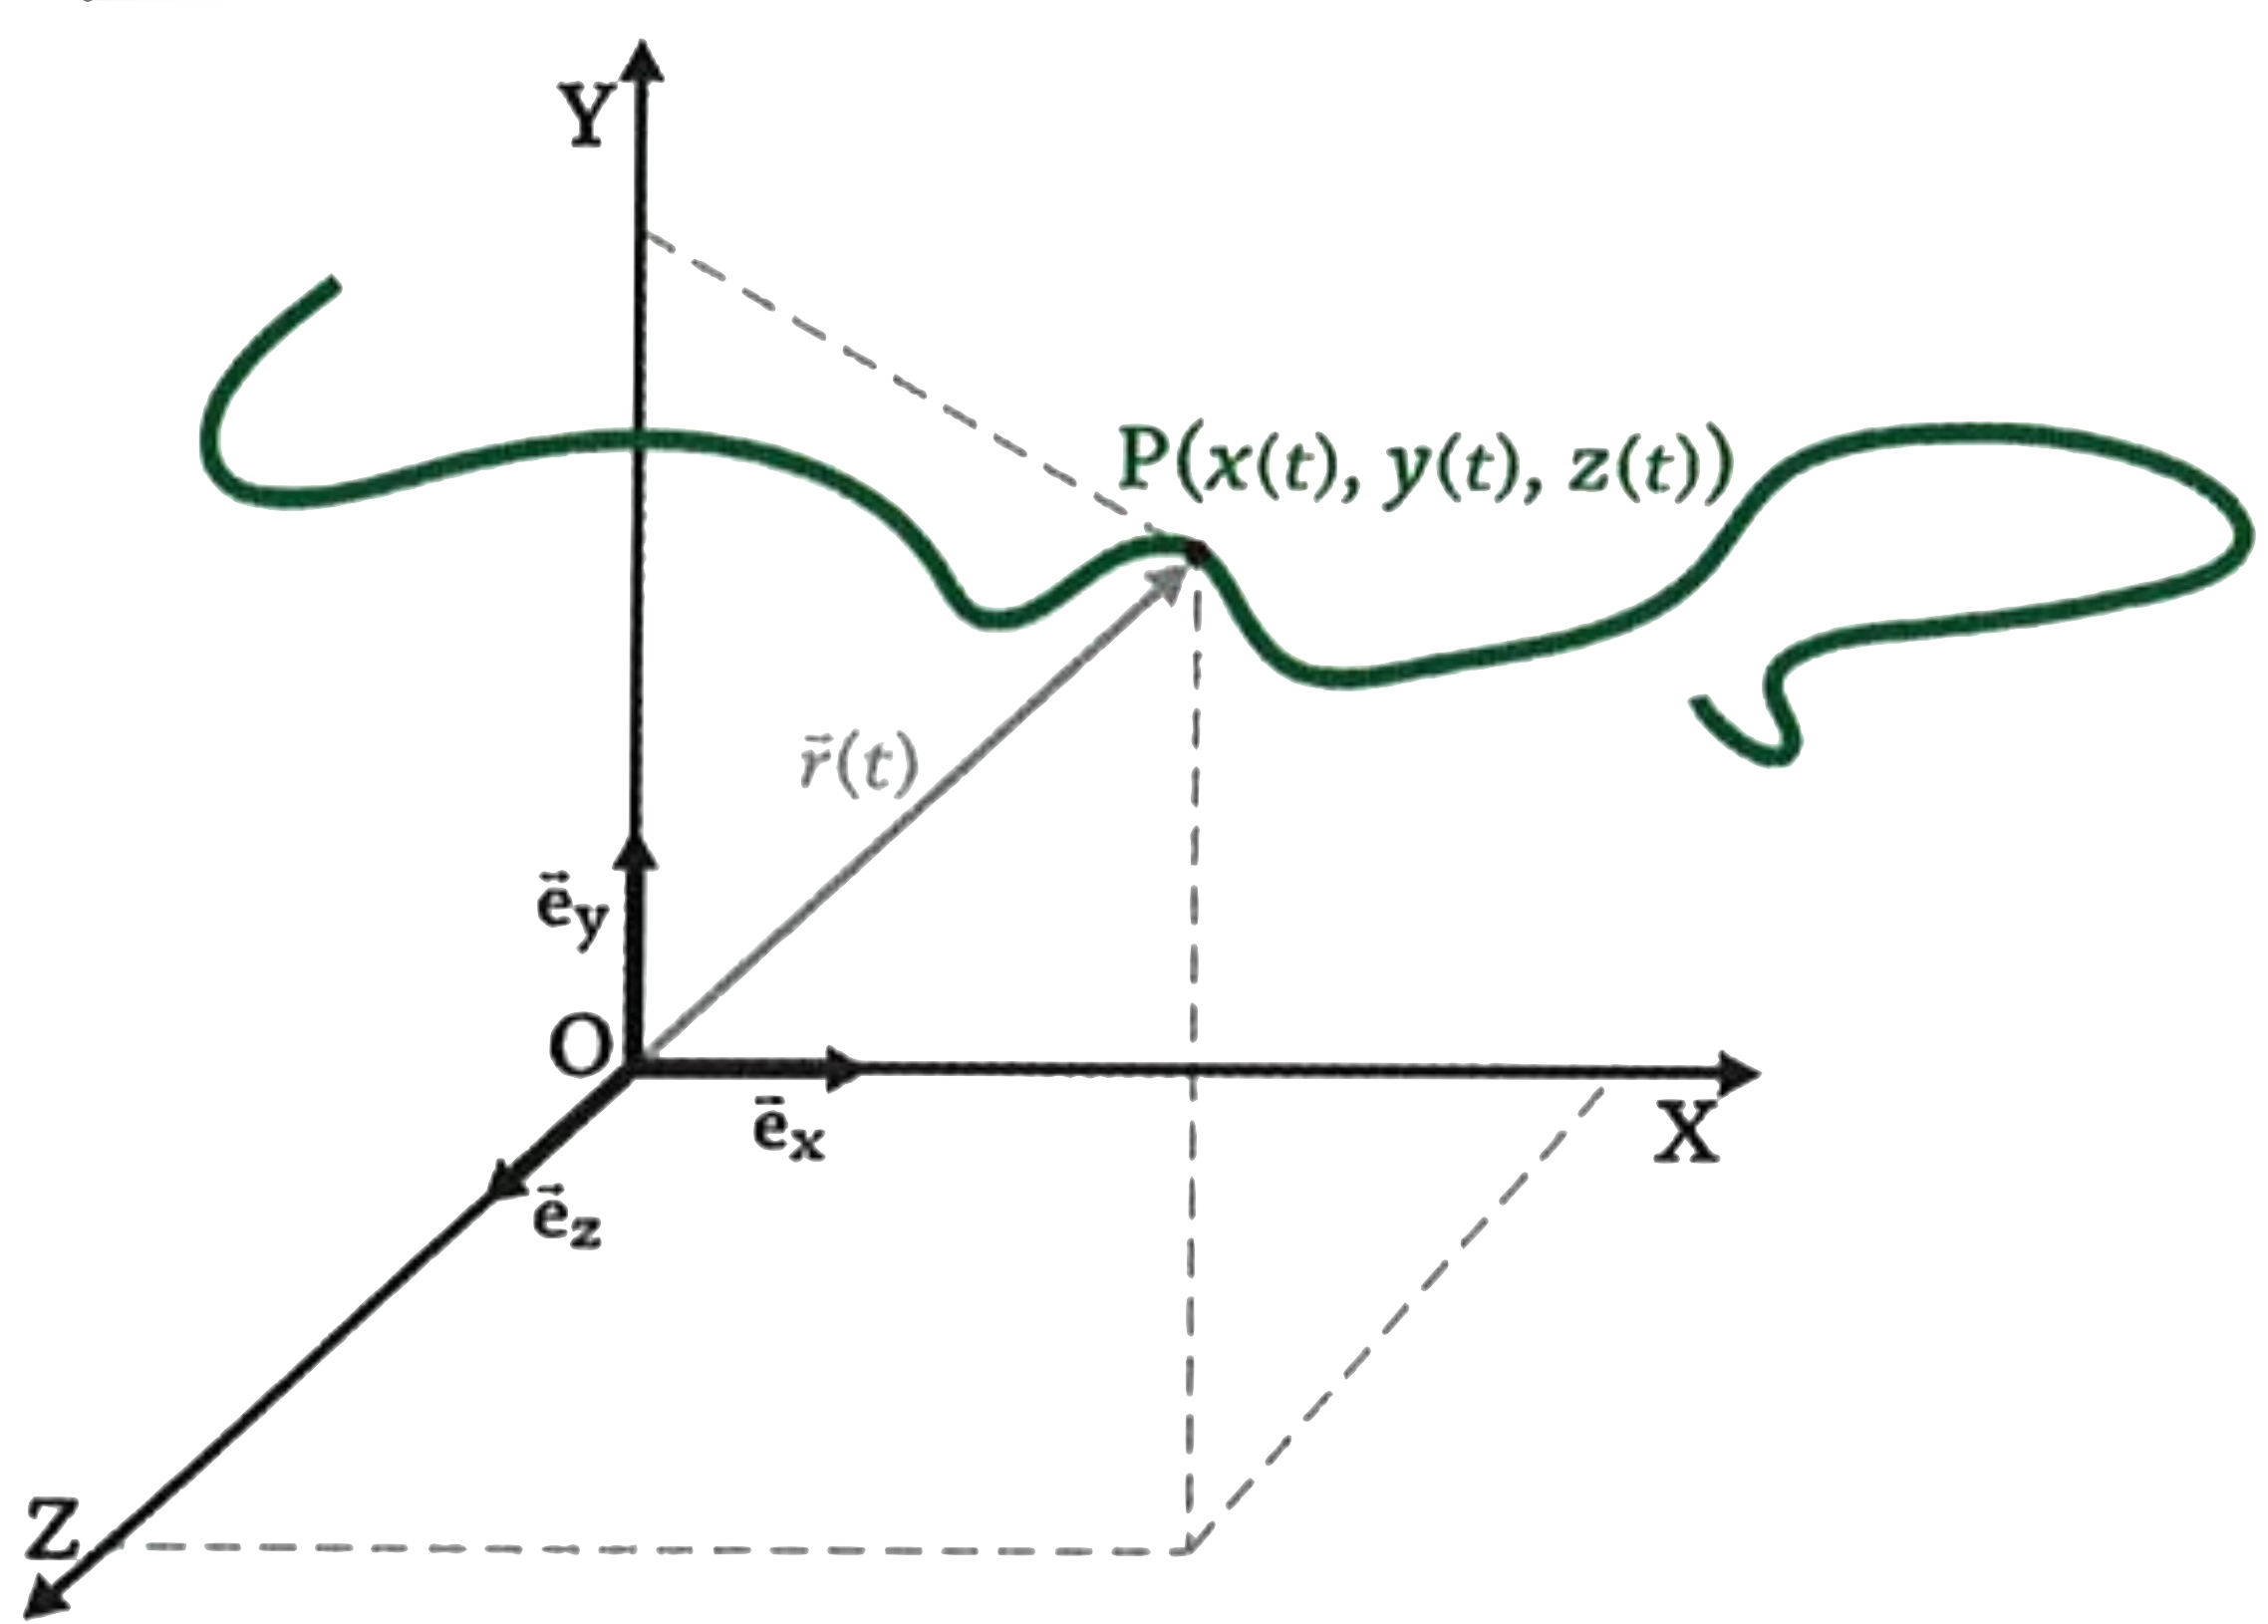
\includegraphics[height=\textheight-3\baselineskip]{plaatsvector-2}
\end{figure}
\end{frame}

\begin{frame}{Plaats}
%\framesubtitle{}
\begin{itemize}
\item<1-> De positie van een object in de ruimte kunnen we beschrijven aan de hand van een punt met co\"ordinaten in een cartesiaans assenstelsel:
\begin{displaymath}
P(x,y)	
\end{displaymath}
\item<2-> De afhankelijkheid van de tijd kunnen we beschrijven a.d.h.v. de tijdsafhankelijkheid van de co\"ordinaten:
\begin{displaymath}
	P(x(t),y(t))
\end{displaymath}
\item<3-> $x(t)$ en $y(t)$ zijn co\"ordinaatsfuncties.
\end{itemize}
\end{frame}

%\begin{frame}{Plaats}
%%\framesubtitle{}
%\begin{itemize}
%\item<1-> De positie van een object in de ruimte kunnen we beschrijven aan de hand van een punt met co\"ordinaten in een cartesiaans assenstelsel:
%\begin{displaymath}
%P(x,y,z)	
%\end{displaymath}
%\item<2-> De afhankelijkheid van de tijd kunnen we beschrijven a.d.h.v. de tijdsafhankelijkheid van de co\"ordinaten:
%\begin{displaymath}
%	P(x(t),y(t),z(t))
%\end{displaymath}
%\item<3-> $x(t),y(t),z(t)$ zijn co\"ordinaatsfuncties.
%\end{itemize}
%\end{frame}




\begin{frame}{Plaatsvector}
%\framesubtitle{}
\begin{itemize}
\item<1-> Een equivalente manier van voorstelling met een plaatsvector:
\begin{eqnarray*}
	\vec{r}
	%\pause
	&=&\vec{r}_x+\vec{r}_y\\
	%\pause
	&=&x\cdot\vec{e}_x+y\cdot\vec{e}_y\\
\end{eqnarray*}	
\item<2-> Met (expliciete) tijdsafhankelijkheid $\vec{r}=\vec{r}(t)$:
\begin{eqnarray*}
	\vec{r}(t)=x(t)\cdot\vec{e}_x+y(t)\cdot\vec{e}_y\\
\end{eqnarray*}	
\end{itemize}
\end{frame}


%\begin{frame}{Plaatsvector}
%%\framesubtitle{}
%\begin{itemize}
%\item<1-> Een equivalente manier van voorstelling met een plaatsvector:
%\begin{eqnarray*}
%	\vec{r}
%	%\pause
%	&=&\vec{r}_x+\vec{r}_y+\vec{r}_z\\
%	%\pause
%	&=&x\cdot\vec{e}_x+y\cdot\vec{e}_y+z\cdot\vec{e}_z\\
%\end{eqnarray*}	
%\item<2-> Met (expliciete) tijdsafhankelijkheid $\vec{r}=\vec{r}(t)$:
%\begin{eqnarray*}
%	\vec{r}(t)=x(t)\cdot\vec{e}_x+y(t)\cdot\vec{e}_y+z(t)\cdot\vec{e}_z\\
%\end{eqnarray*}	
%\end{itemize}
%\end{frame}



\subsection{Verplaatsing}

\begin{frame}{Verplaatsing vs. afgelegde weg}
\begin{figure}
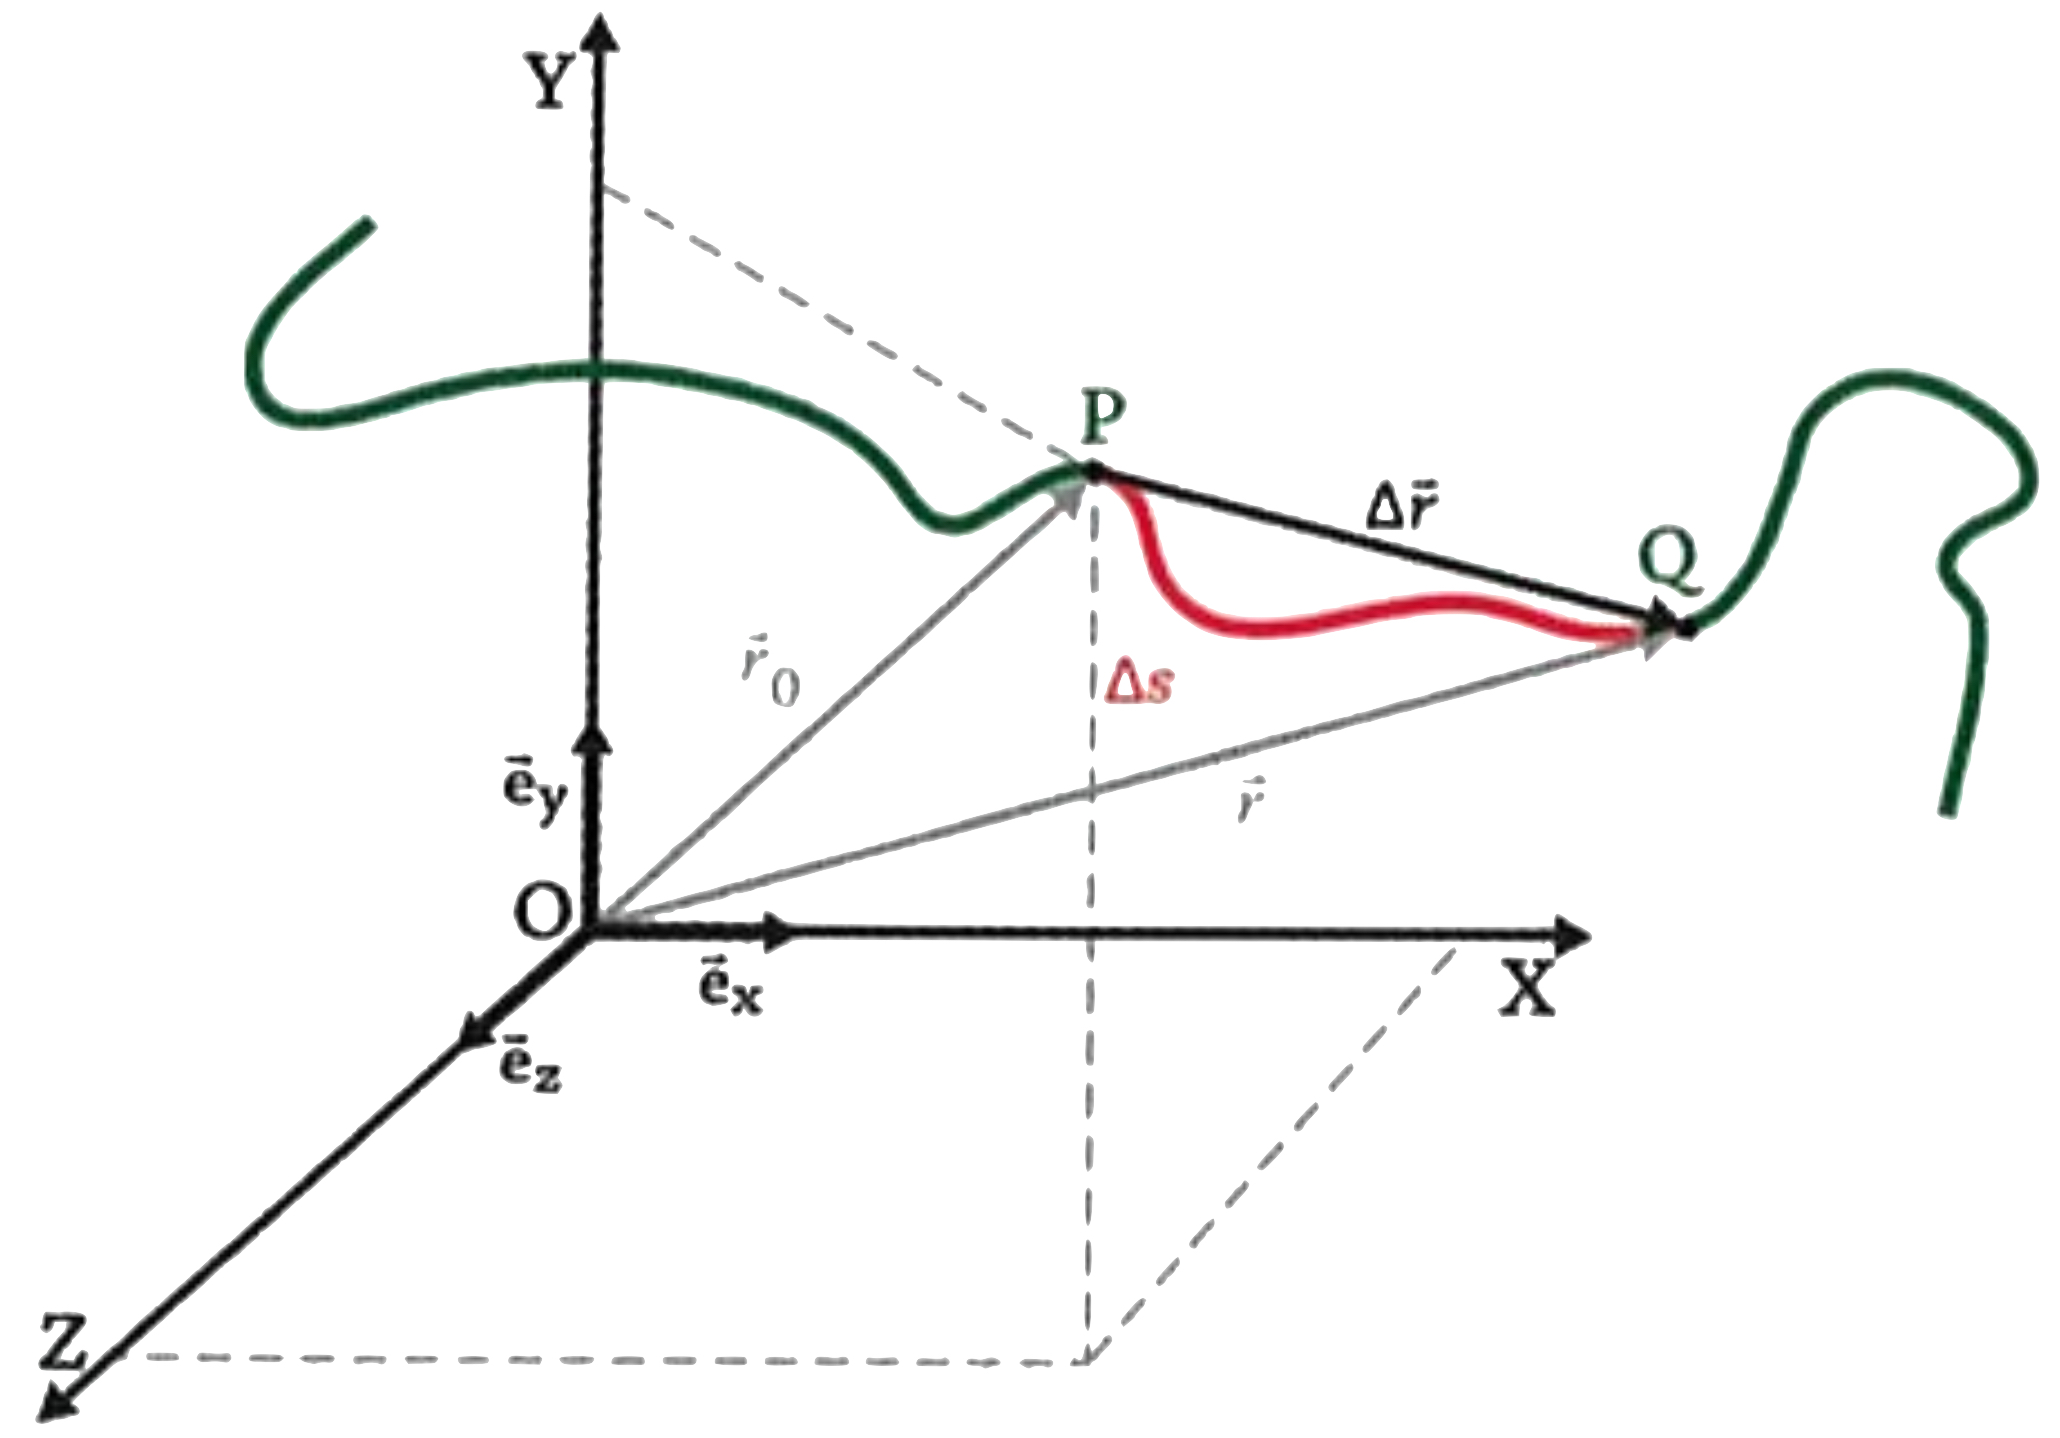
\includegraphics[height=\textheight-3\baselineskip]{verplaatsing-2}
\end{figure}
\end{frame}

\note[itemize]{
\item plaatsvector om verplaatsing als vector te kunnen defini\"eren. Niet alleen de grootte van de verplaatsing doet er toe. 
}


\begin{frame}{Verplaatsing}
%\framesubtitle{}	
\begin{itemize}[<+->]	
\item Verplaatsing
\begin{displaymath}
	\vec{\Delta r}=\vec{r}_2-\vec{r}_1
\end{displaymath}
\item Grootte van de verplaatsing
\begin{displaymath}
	\Delta r=|| \vec{\Delta r} ||
\end{displaymath}
\item Afgelegde weg
\begin{displaymath}
	\Delta s
\end{displaymath}
\end{itemize}
\end{frame}

\note[itemize]{
\item Fysische grootheden om een verandering in de ruimte weer te kunnen geven.
\item Vectori\"ele vs scalaire grootheid
\item eenheid meter
\item lengte van de route/baan/het parcours
\item Numerieke waarden kan samenvallen/verschillen
}




\usebackgroundtemplate{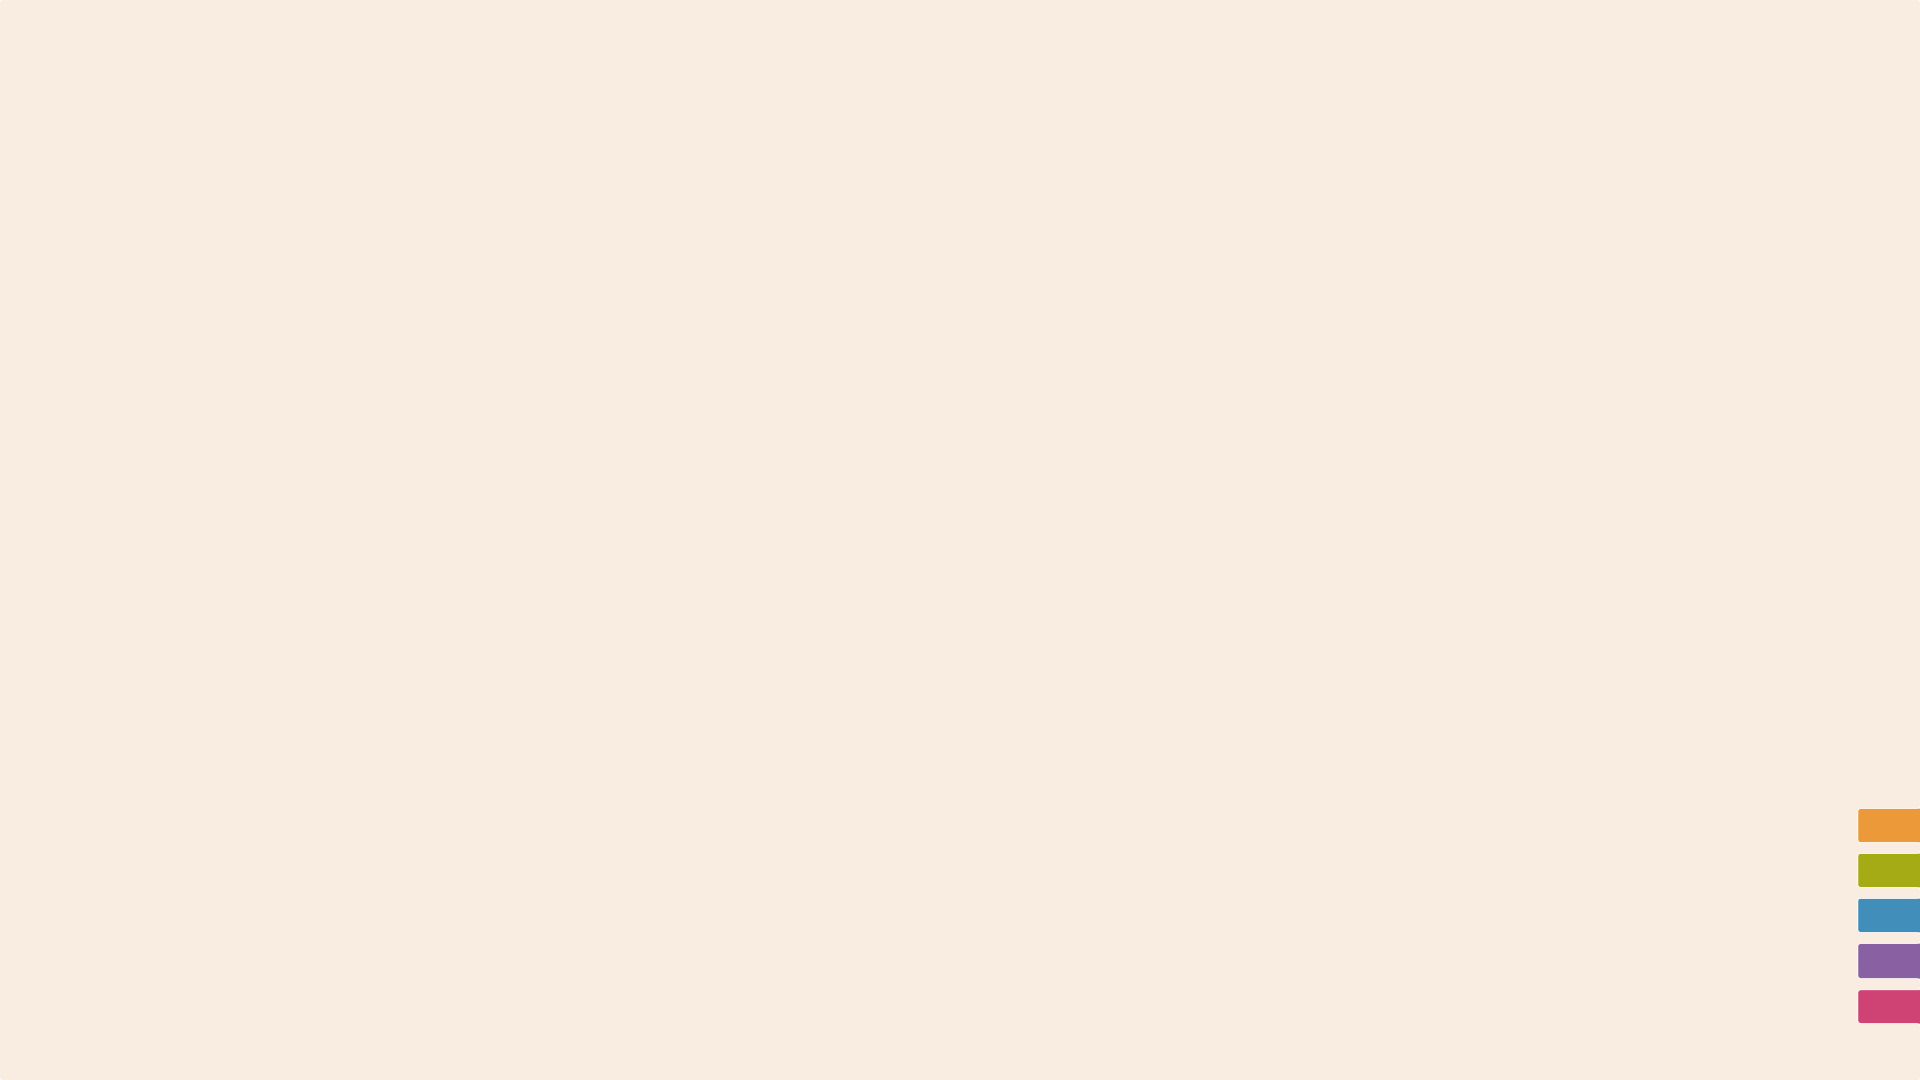
\includegraphics[width=\paperwidth,height=\paperheight]{achtergrond22n_FV}}

\begin{frame}{Voorbeeld 3 p. 13}
\begin{figure}	
\centering
\includegraphics[height=.8\textheight]{voorbeeld_3}
%\includegraphics[width=.9\textwidth]{voorbeeld_3}
\end{figure}
\end{frame}

\note[itemize]{
\item Een van de banen moet blijkbaar \SI{400}{m} lang zijn \ldots
\item Afgelegde weg/weg langs de baan gemeten/lengte van het parcours
}


\begin{frame}{Voorbeeld 3 p. 13}
\begin{eqnarray*}
\Delta\vec{r}&=&\vec{r}-\vec{r_0}\\
\pause
&=&(x\cdot\noindent{\color{blue}{\vec{e}_x}}+y\cdot\noindent{\color{teal}{\vec{e}_y}})-(x_0\cdot\noindent{\color{blue}{\vec{e}_x}}+y_0\cdot\noindent{\color{teal}{\vec{e}_y}})\\
\pause
&=&(x-x_0)\cdot\noindent{\color{blue}{\vec{e}_x}}+(y-y_0)\cdot\noindent{\color{teal}{\vec{e}_y}}\\
\pause
&=&(100-20)\cdot\noindent{\color{blue}{\vec{e}_x}}+(0-70)\cdot\noindent{\color{teal}{\vec{e}_y}}\\
\pause
&=&80\cdot\noindent{\color{blue}{\vec{e}_x}}-70\cdot\noindent{\color{teal}{\vec{e}_y}}\\
\end{eqnarray*}
\end{frame}

\note[itemize]{
\item Een van de banen moet blijkbaar \SI{400}{m} lang zijn \ldots
\item Afgelegde weg/weg langs de baan gemeten/lengte van het parcours
\item Wat zouden we als definitie kunnen nemen voor de gemiddelde snelheid \ldots?
}



\usebackgroundtemplate{
\includegraphics[width=\paperwidth,height=\paperheight]{achtergrond22n}}


%\begin{frame}{Tijdsduur}
%\framesubtitle{Tijdsduur, tijdsinterval, tijdsverloop}\begin{displaymath}
%	\Delta t=t_2-t_1
%\end{displaymath}
%\end{frame}


\subsection{Snelheid}


\begin{frame}{Gemiddelde snelheid}
%\framesubtitle{}
\begin{block}{}
De gemiddelde snelheid over een tijdsinterval $\Delta t$ wordt gedefinieerd door:
\begin{displaymath}
	\vec{v}_{\text{gem}}=\frac{\vec{\Delta r}}{\Delta t}
\end{displaymath}
\end{block}
%\pause
De eenheid van de grootte van de (gemiddelde) snelheid is $\SI{}{m/s}$.
\end{frame}

\note[itemize]{
\item Figuur van gemiddelde snelheidsvector maken \ldots
}



\begin{frame}{Ogenblikkelijke snelheid}
%\framesubtitle{}
\begin{figure}
\href{run:./media/Horizontale_worp_num.gif}{%
\includegraphics[height=\textheight-3\baselineskip]{Horizontale_worp}
}
\end{figure}
\end{frame}




\begin{frame}{Ogenblikkelijke snelheid}
%\framesubtitle{}
\begin{block}{}
De (ogenblikkelijke) snelheid in functie van de tijd wordt gedefinieerd door:
\begin{eqnarray*}
	\vec{v}&=&\lim_{\Delta t\to0}\frac{\vec{\Delta r}}{\Delta t}\\
	%\pause
	&=&\frac{d\vec{r}}{dt}
\end{eqnarray*}
\end{block}
\end{frame}


\begin{frame}{Ogenblikkelijke snelheid}
%\framesubtitle{}

\begin{eqnarray*}
	\vec{v}\,=\,\lim_{\Delta t\to0}\frac{\vec{\Delta r}}{\Delta t}
	&=&\lim_{t\to t_0}\frac{(x-x_0)\cdot\vec{e}_x+(y-y_0)\cdot\vec{e}_y}{t-t_0}\\
	\pause
	&=&\lim_{t\to t_0}\left(\frac{x-x_0}{t-t_0}\cdot\vec{e}_x+\frac{y-y_0}{t-t_0}\cdot\vec{e}_y\right)\\
	\pause
	&=&\lim_{t\to t_0}\left(\frac{x-x_0}{t-t_0}\cdot\vec{e}_x\right)+\left(\frac{y-y_0}{t-t_0}\cdot\vec{e}_y\right)\\
	\pause
	&=&\lim_{t\to t_0}\left(\frac{x-x_0}{t-t_0}\right)\cdot\vec{e}_x+\left(\frac{y-y_0}{t-t_0}\right)\cdot\vec{e}_y\\
	\pause
	&=&\frac{dx}{dt}\cdot\vec{e}_x+\frac{dy}{dt}\cdot\vec{e}_y\\
	\pause
	&=&v_x\cdot\vec{e}_x+v_y\cdot\vec{e}_y
\end{eqnarray*}
\end{frame}



%\begin{frame}{Ogenblikkelijke snelheid}
%\begin{figure}
%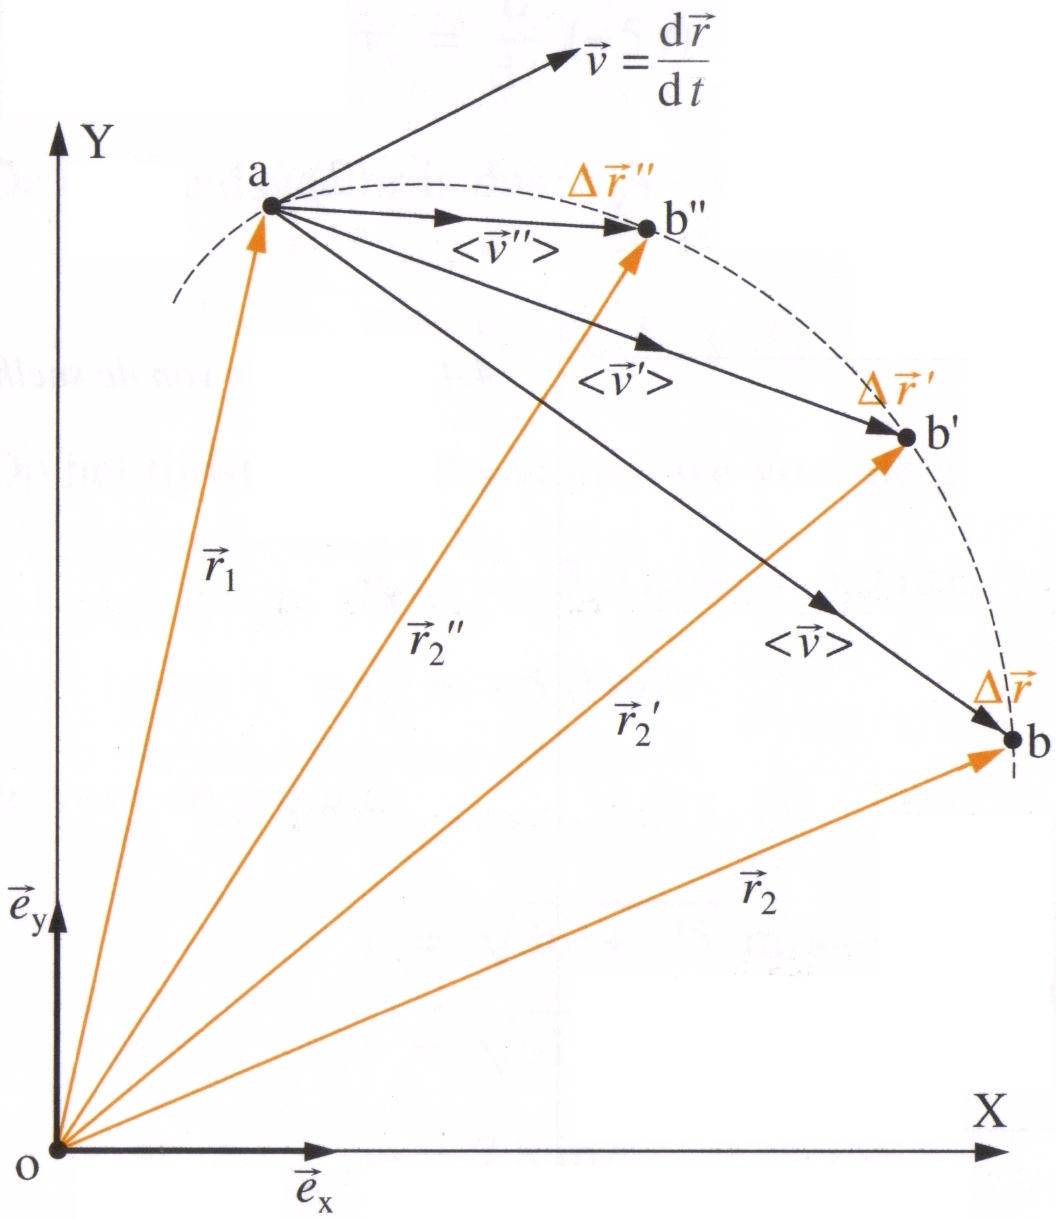
\includegraphics[height=\textheight-3\baselineskip]{gem_snelheidsvector}
%\end{figure}
%\end{frame}

\begin{frame}{Ogenblikkelijke snelheid}
%\framesubtitle{}
De snelheid is een vector en dus te ontbinden in componenten:
\begin{eqnarray*}	
\vec{v}&=&\vec{v}_x+ \vec{v}_y\\
%\pause
&=&v_x\cdot\vec{e}_x+v_y\cdot\vec{e}_y\\
%\pause
&=&\frac{dx}{dt}\cdot\vec{e}_x+\frac{dy}{dt}\cdot\vec{e}_y\\
\end{eqnarray*}
\end{frame}

\note[itemize]{
\item Limiet uitschrijven en som van limieten maken. Gaat over limietvector.
\item Definitie geeft ons een snelheidsvector zoals we willen, met componenten en betekenis overeenkomstig onze intu\"itie die de beweging spontaan opknipt in deelaspecten.
}

\usebackgroundtemplate{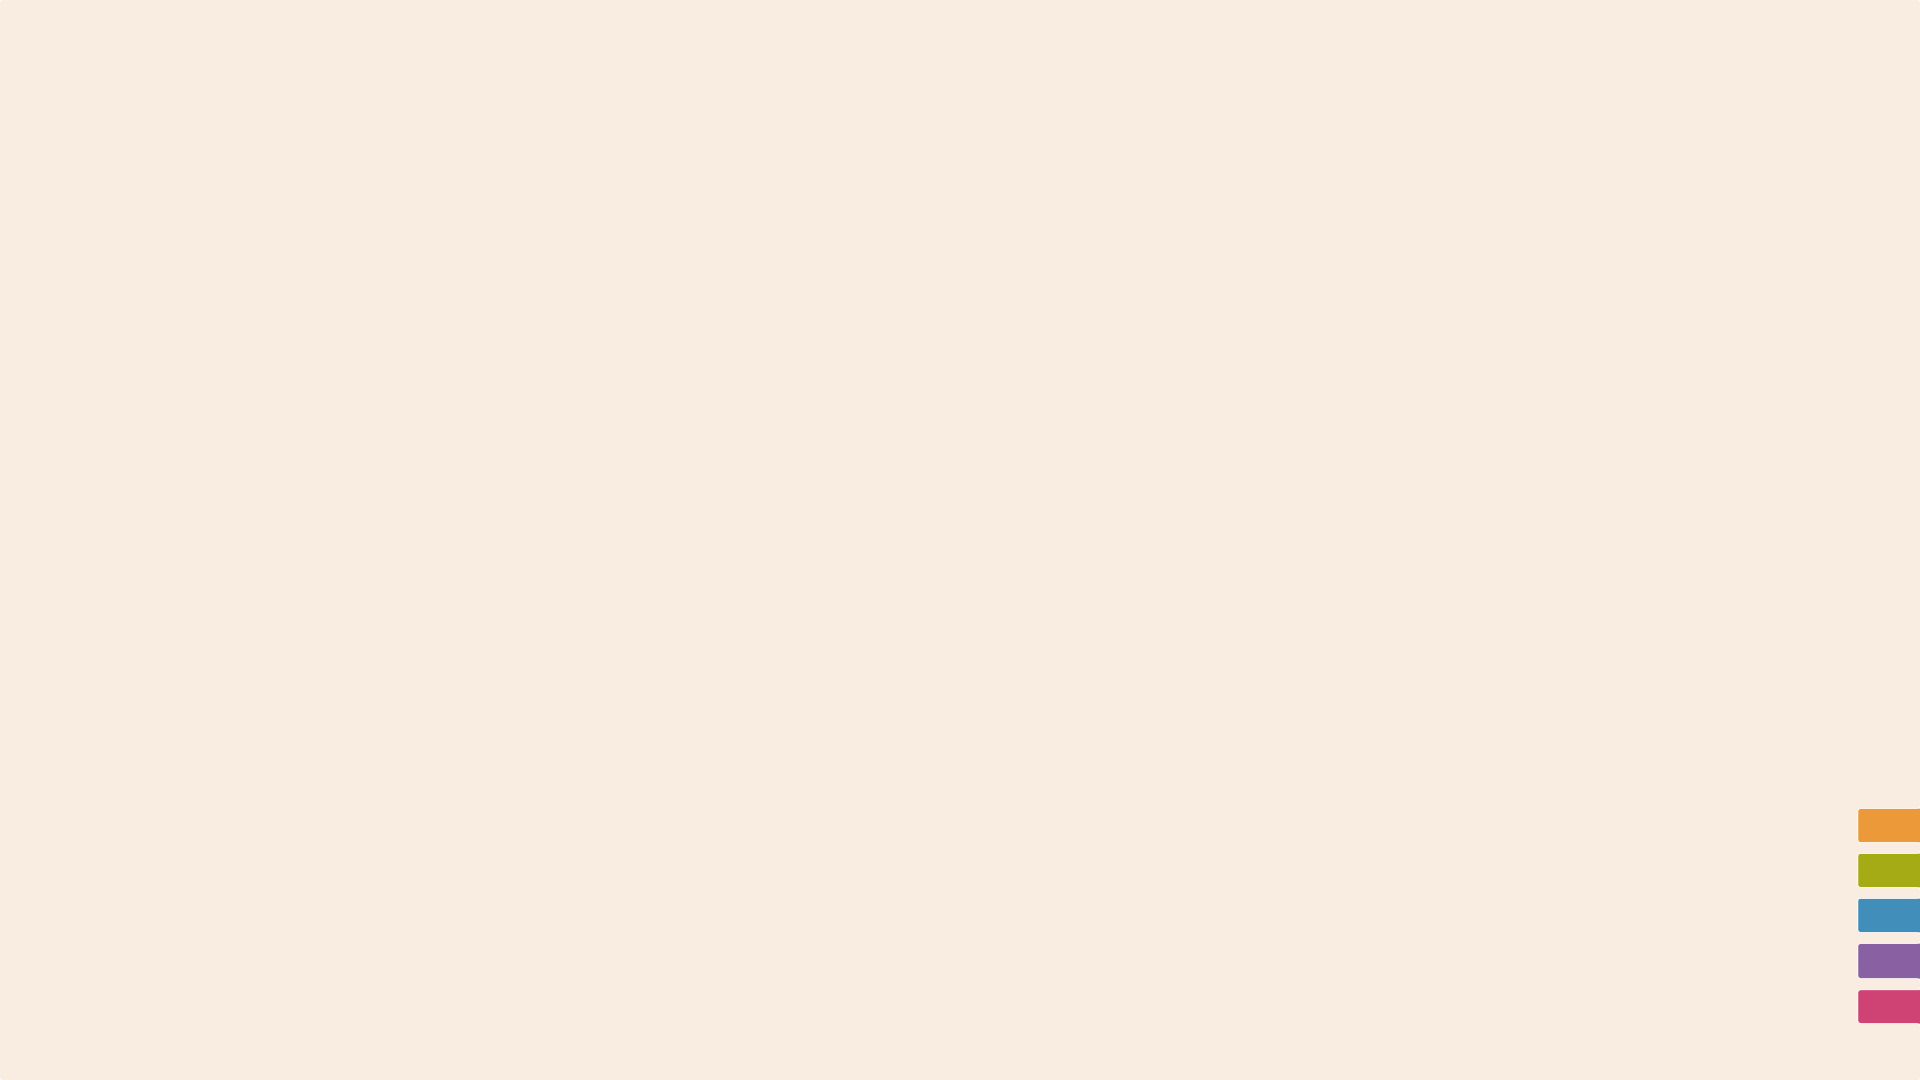
\includegraphics[width=\paperwidth,height=\paperheight]{achtergrond22n_FV}}

\begin{frame}{Voorbeeld 5 p. 17}
\begin{figure}
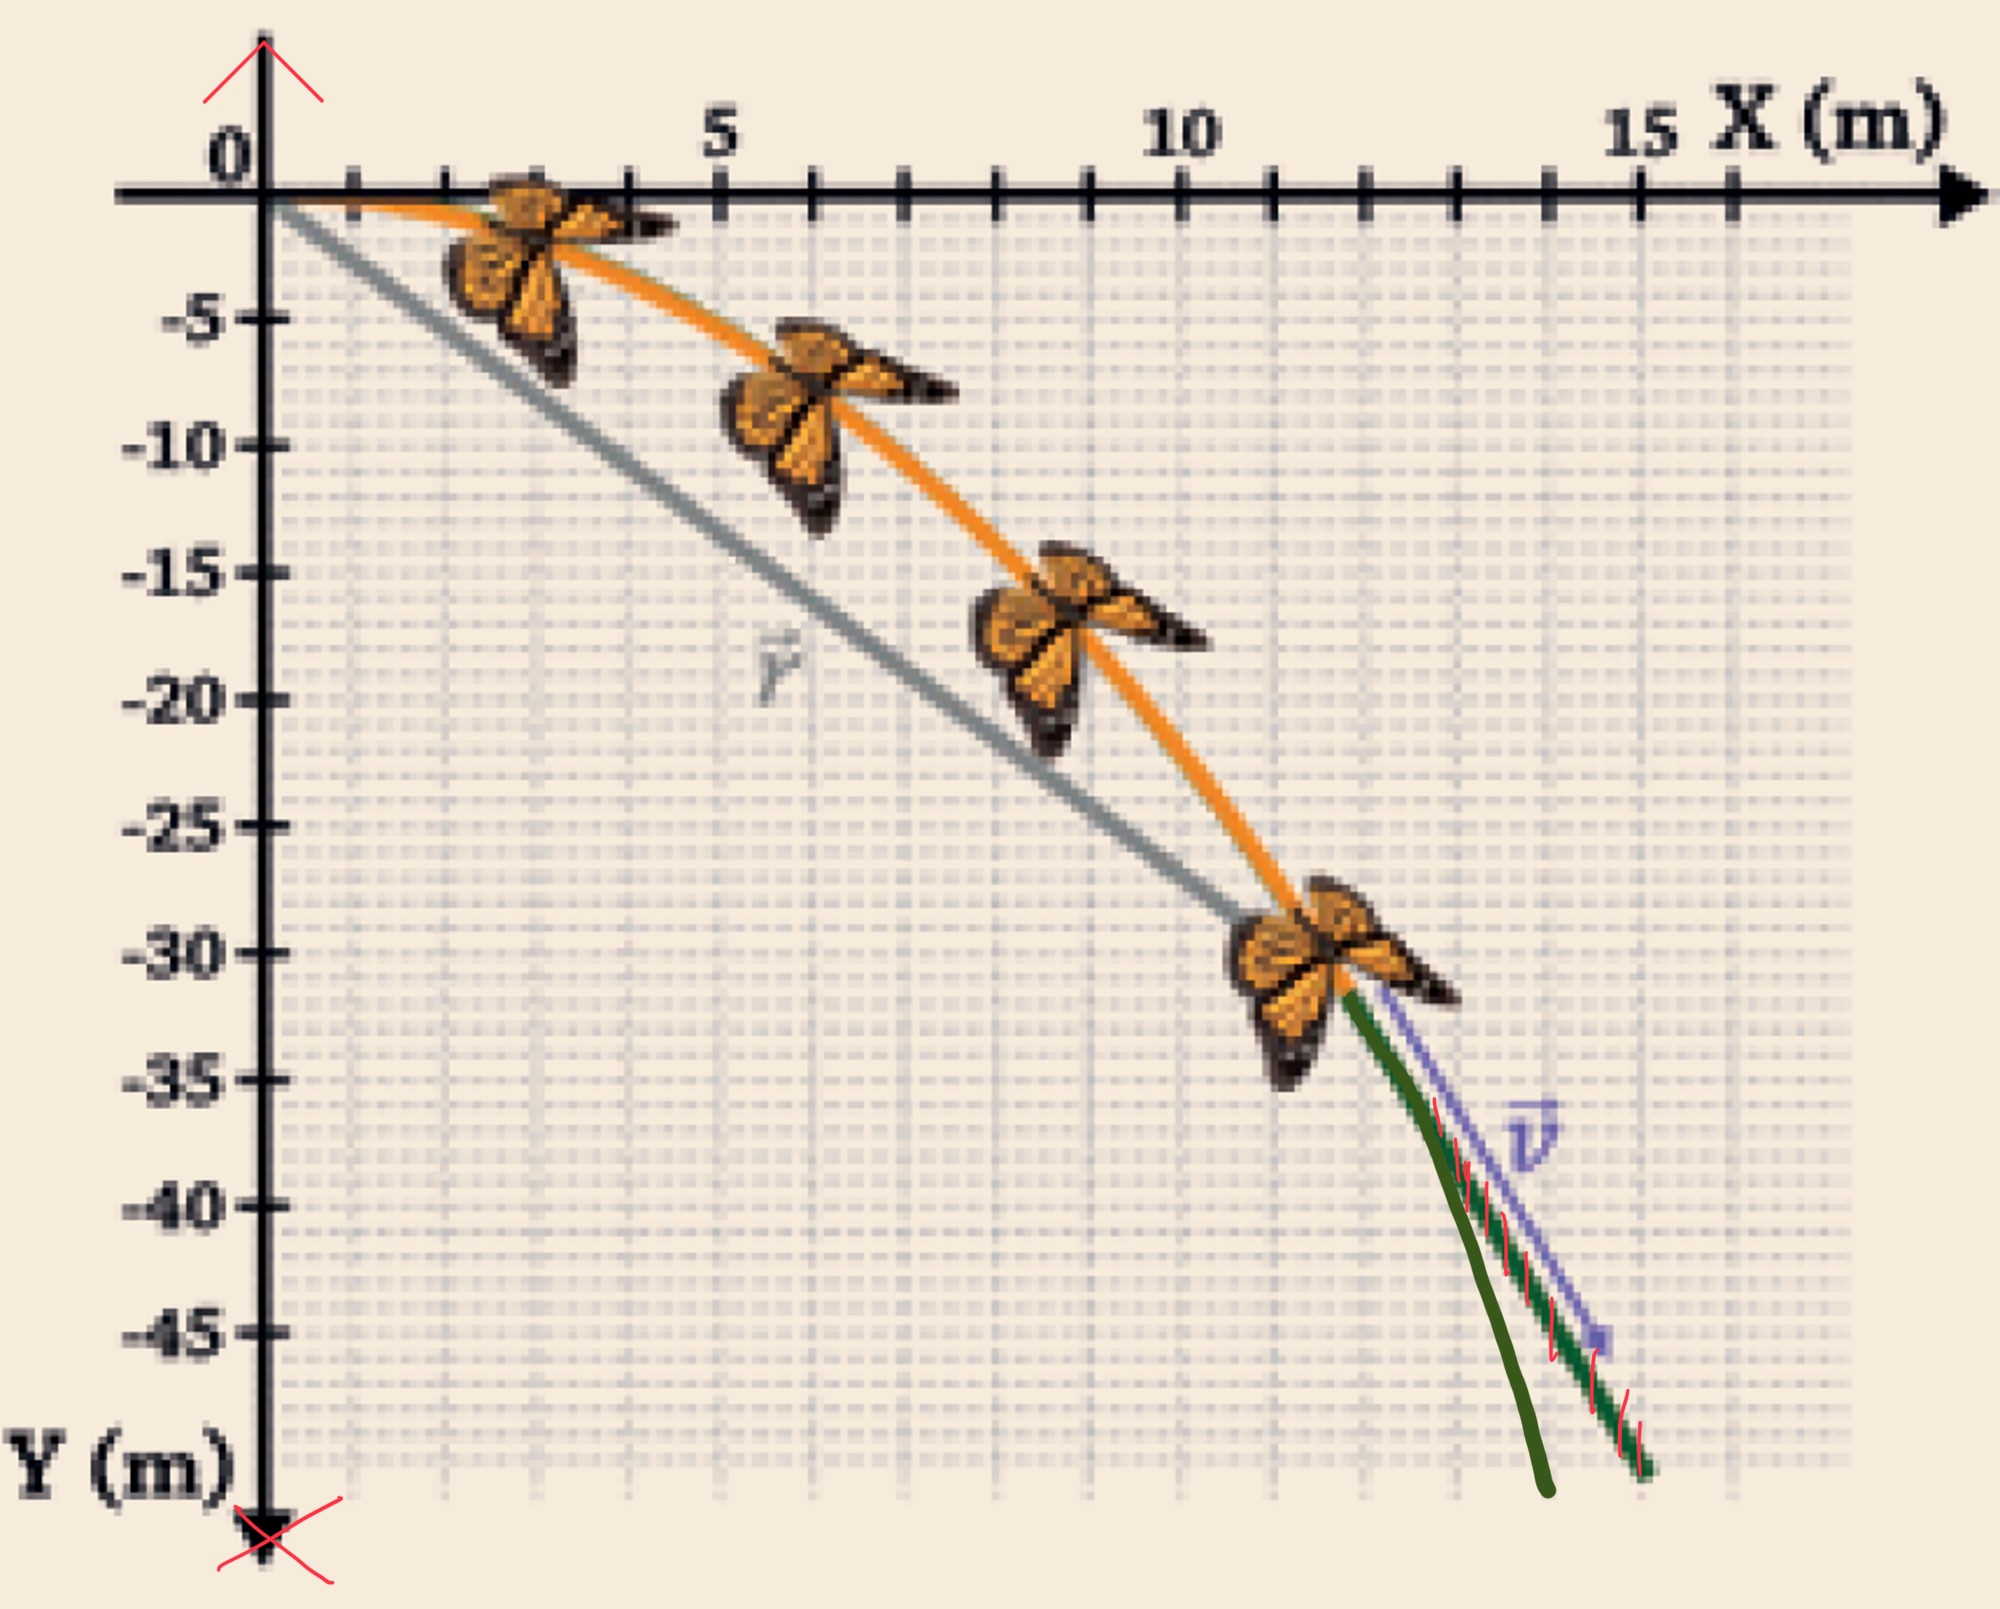
\includegraphics[height=\textheight-3\baselineskip]{voorbeeld_5}
\end{figure}
\end{frame}

\note[itemize]{
\item Zelfstudie
}

\usebackgroundtemplate{
\includegraphics[width=\paperwidth,height=\paperheight]{achtergrond22n}}



\subsection{Versnelling}

%\begin{frame}{Versnelling}
%\framesubtitle{§1.2 p. 21}
%\href{run:./apps/hodograaf.ggb}{Hodograaf}
%\end{frame}

\begin{frame}{Versnelling}
%\framesubtitle{}
\begin{figure}
\href{run:./media/ProjectilefromaMovingTruckDemo.webm}{%
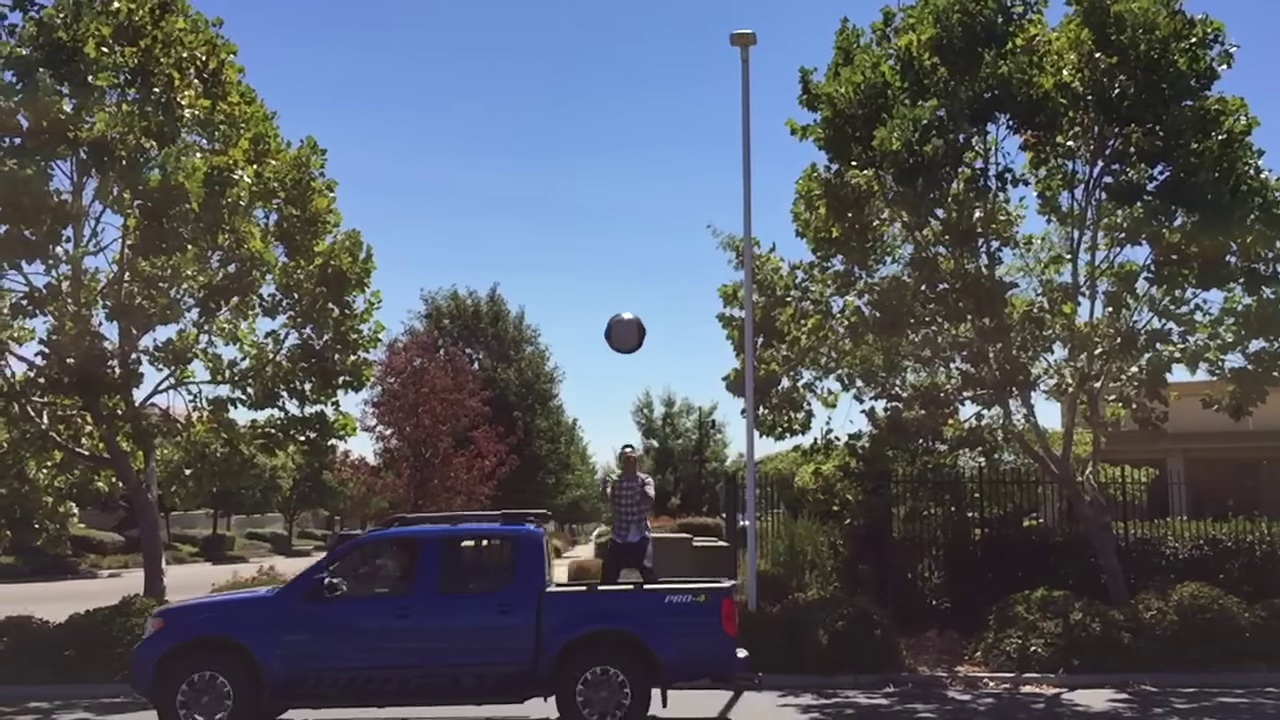
\includegraphics[height=\textheight-3\baselineskip]{vlcsnap-2022-09-21-21h28m34s708}
}
\end{figure}
\end{frame}

\begin{frame}{Gemiddelde versnelling}
%\framesubtitle{§1.2 p. 21}
\begin{block}{}
De gemiddelde versnelling over een tijdsinterval $\Delta t$ wordt gedefineerd door:
\begin{displaymath}
	\vec{a}_{\text{gem}}=\frac{\vec{\Delta v}}{\Delta t}
\end{displaymath}
\end{block}
%\pause
De eenheid van de grootte van de (gemiddelde) versnelling is $\SI{}{m/s^2}$.
\end{frame}


\begin{frame}{Ogenblikkelijke versnelling}
%\framesubtitle{}
\begin{figure}
\href{run:./media/Horizontale_worp_deltav.gif}{%
\includegraphics[height=\textheight-3\baselineskip]{Horizontale_worp_deltav}
}
\end{figure}
\end{frame}



\begin{frame}{Ogenblikkelijke versnelling}
%\framesubtitle{}
\begin{block}{}
De (ogenblikkelijke) versnelling in functie van de tijd wordt gegeven door:
\begin{eqnarray*}
	\vec{a}&=&\lim_{\Delta t\to0}\frac{\vec{\Delta v}}{\Delta t}\\
	%\pause
	&=&\frac{d\vec{v}}{dt}
\end{eqnarray*}
\end{block}
%\pause
\begin{itemize}
  \item<1-> Opmerking: de versnelling is ook de tweede afgeleide van de plaatsvector.
  \item<2-> Notatie: $\displaystyle\vec{a}=\frac{d\vec{v}}{dt}= \frac{d^2\vec{r}}{dt^2}$.
\end{itemize}
\end{frame}

\begin{frame}{Ogenblikkelijke versnelling}
%\framesubtitle{}
De versnelling is een vector en dus te ontbinden in componenten:
\begin{eqnarray*}	
\vec{a}&=&\vec{a}_x+ \vec{a}_y\\
%\pause
&=&a_x\cdot\vec{e}_x+a_y\cdot\vec{e}_y\\
%\pause
&=&\frac{d^2x}{dt^2}\cdot\vec{e}_x+\frac{d^2y}{dt^2}\cdot\vec{e}_y\\
\end{eqnarray*}
\end{frame}



\subsection{Oefeningen}


\usebackgroundtemplate{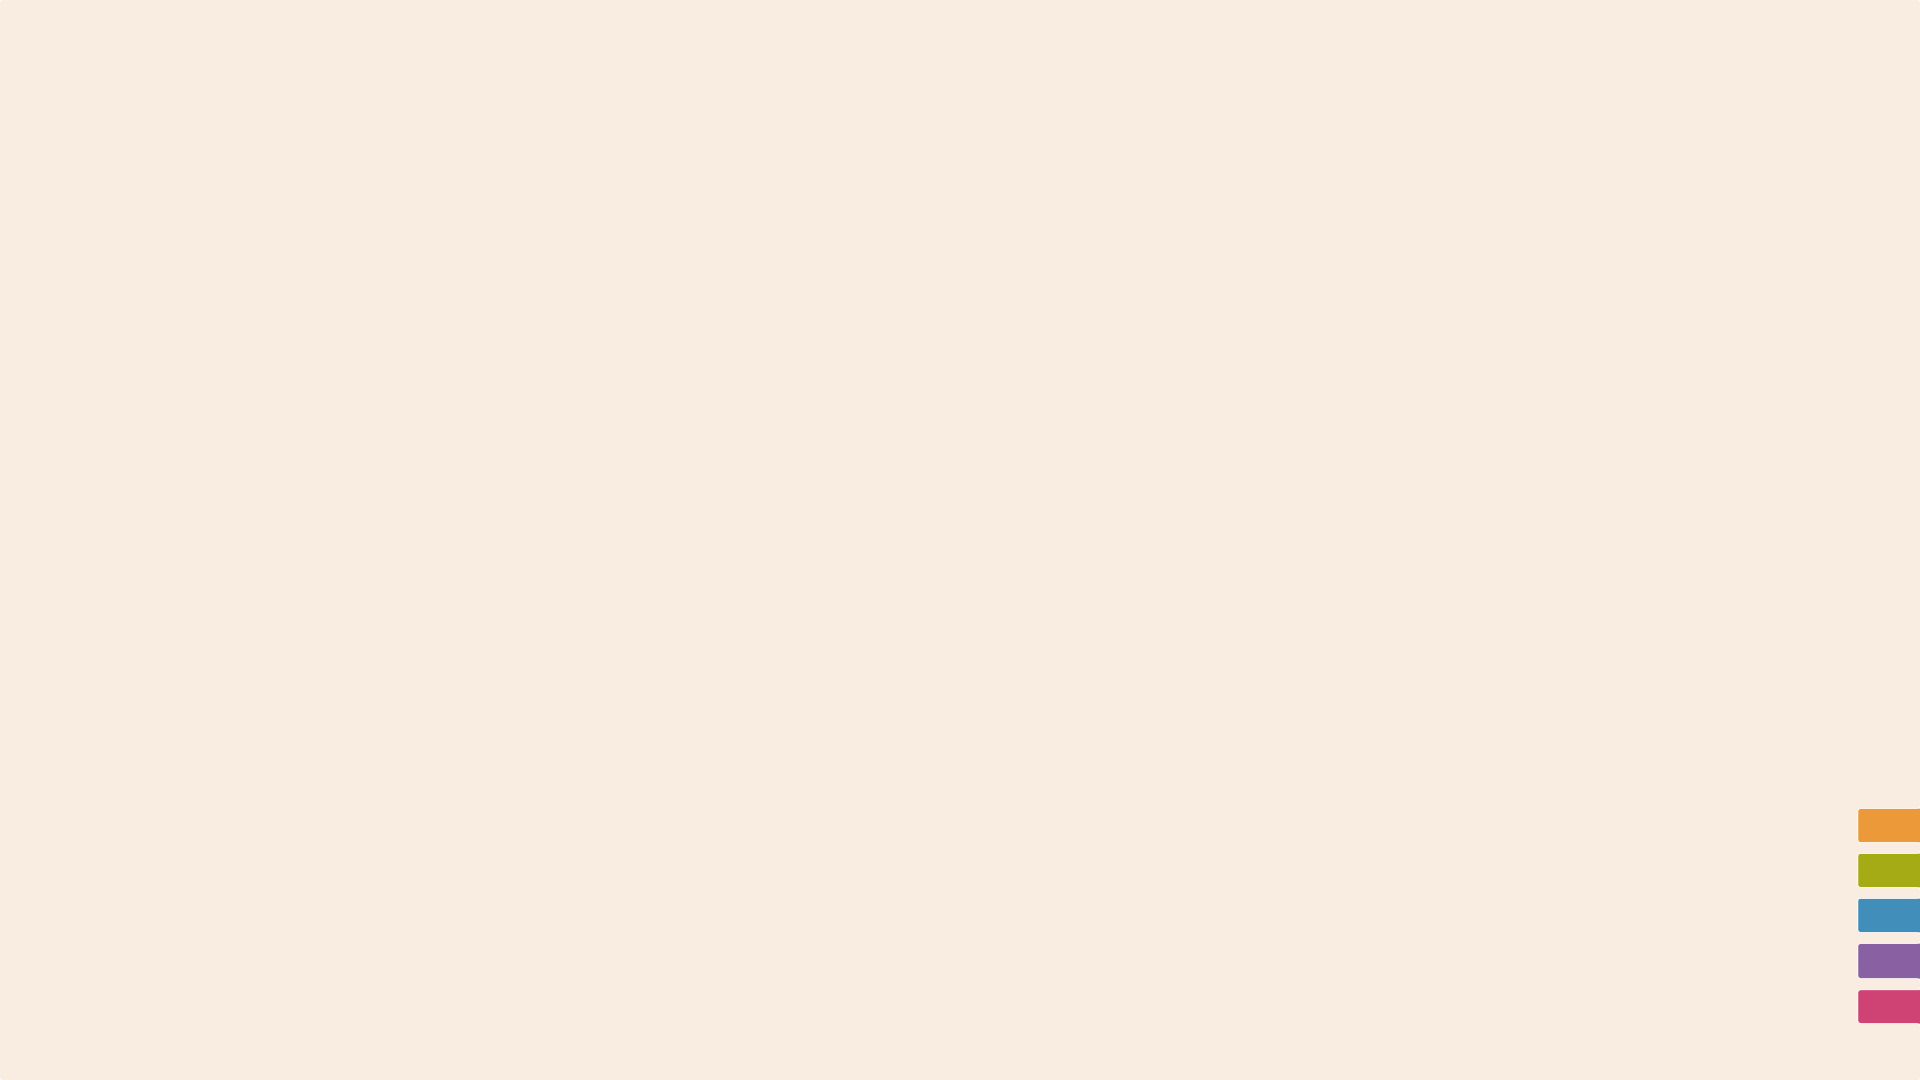
\includegraphics[width=\paperwidth,height=\paperheight]{achtergrond22n_FV}}

%\begin{frame}
%	\frametitle{Voorbeeldoefening}
%	\framesubtitle{cf. 16 p. 88}
%    
%    Een veerman tracht een stromende rivier loodrecht over te roeien. Hij slaagt erin ten opzicht van het water een snelheid van \SI{2,00}{m/s} te ontwikkelen -- de stroomsnelheid is \SI{1,25}{m/s}. Als de rivier \SI{150}{m} breed is, bereken dan
%    
%    \begin{enumerate}
%    	\item onder welke hoek ten opzichte van de loodlijn op de oever hij steeds moet blijven roeien;
%    	\item in hoeveel tijd hij de overzijde bereikt.
%    \end{enumerate}
%    
%\end{frame}
%
%
%\begin{frame}
%\frametitle{Voorbeeldoefening}
%\framesubtitle{cf. 16 p. 88}
%\begin{columns}[T]
%    \begin{column}{0.5\textwidth}
%        Een veerman tracht een stromende rivier loodrecht over te roeien. Hij slaagt erin ten opzicht van het water een snelheid van \SI{2,00}{m/s} te ontwikkelen -- de stroomsnelheid is \SI{1,25}{m/s}. Als de rivier \SI{150}{m} breed is, bereken dan
%        \begin{enumerate}
%        	\item onder welke hoek ten opzichte van de loodlijn op de oever hij steeds moet blijven roeien;
%        	\item in hoeveel tijd hij de overzijde bereikt.
%        \end{enumerate}
%    \end{column}
%    \begin{column}{0.5\textwidth}
%    	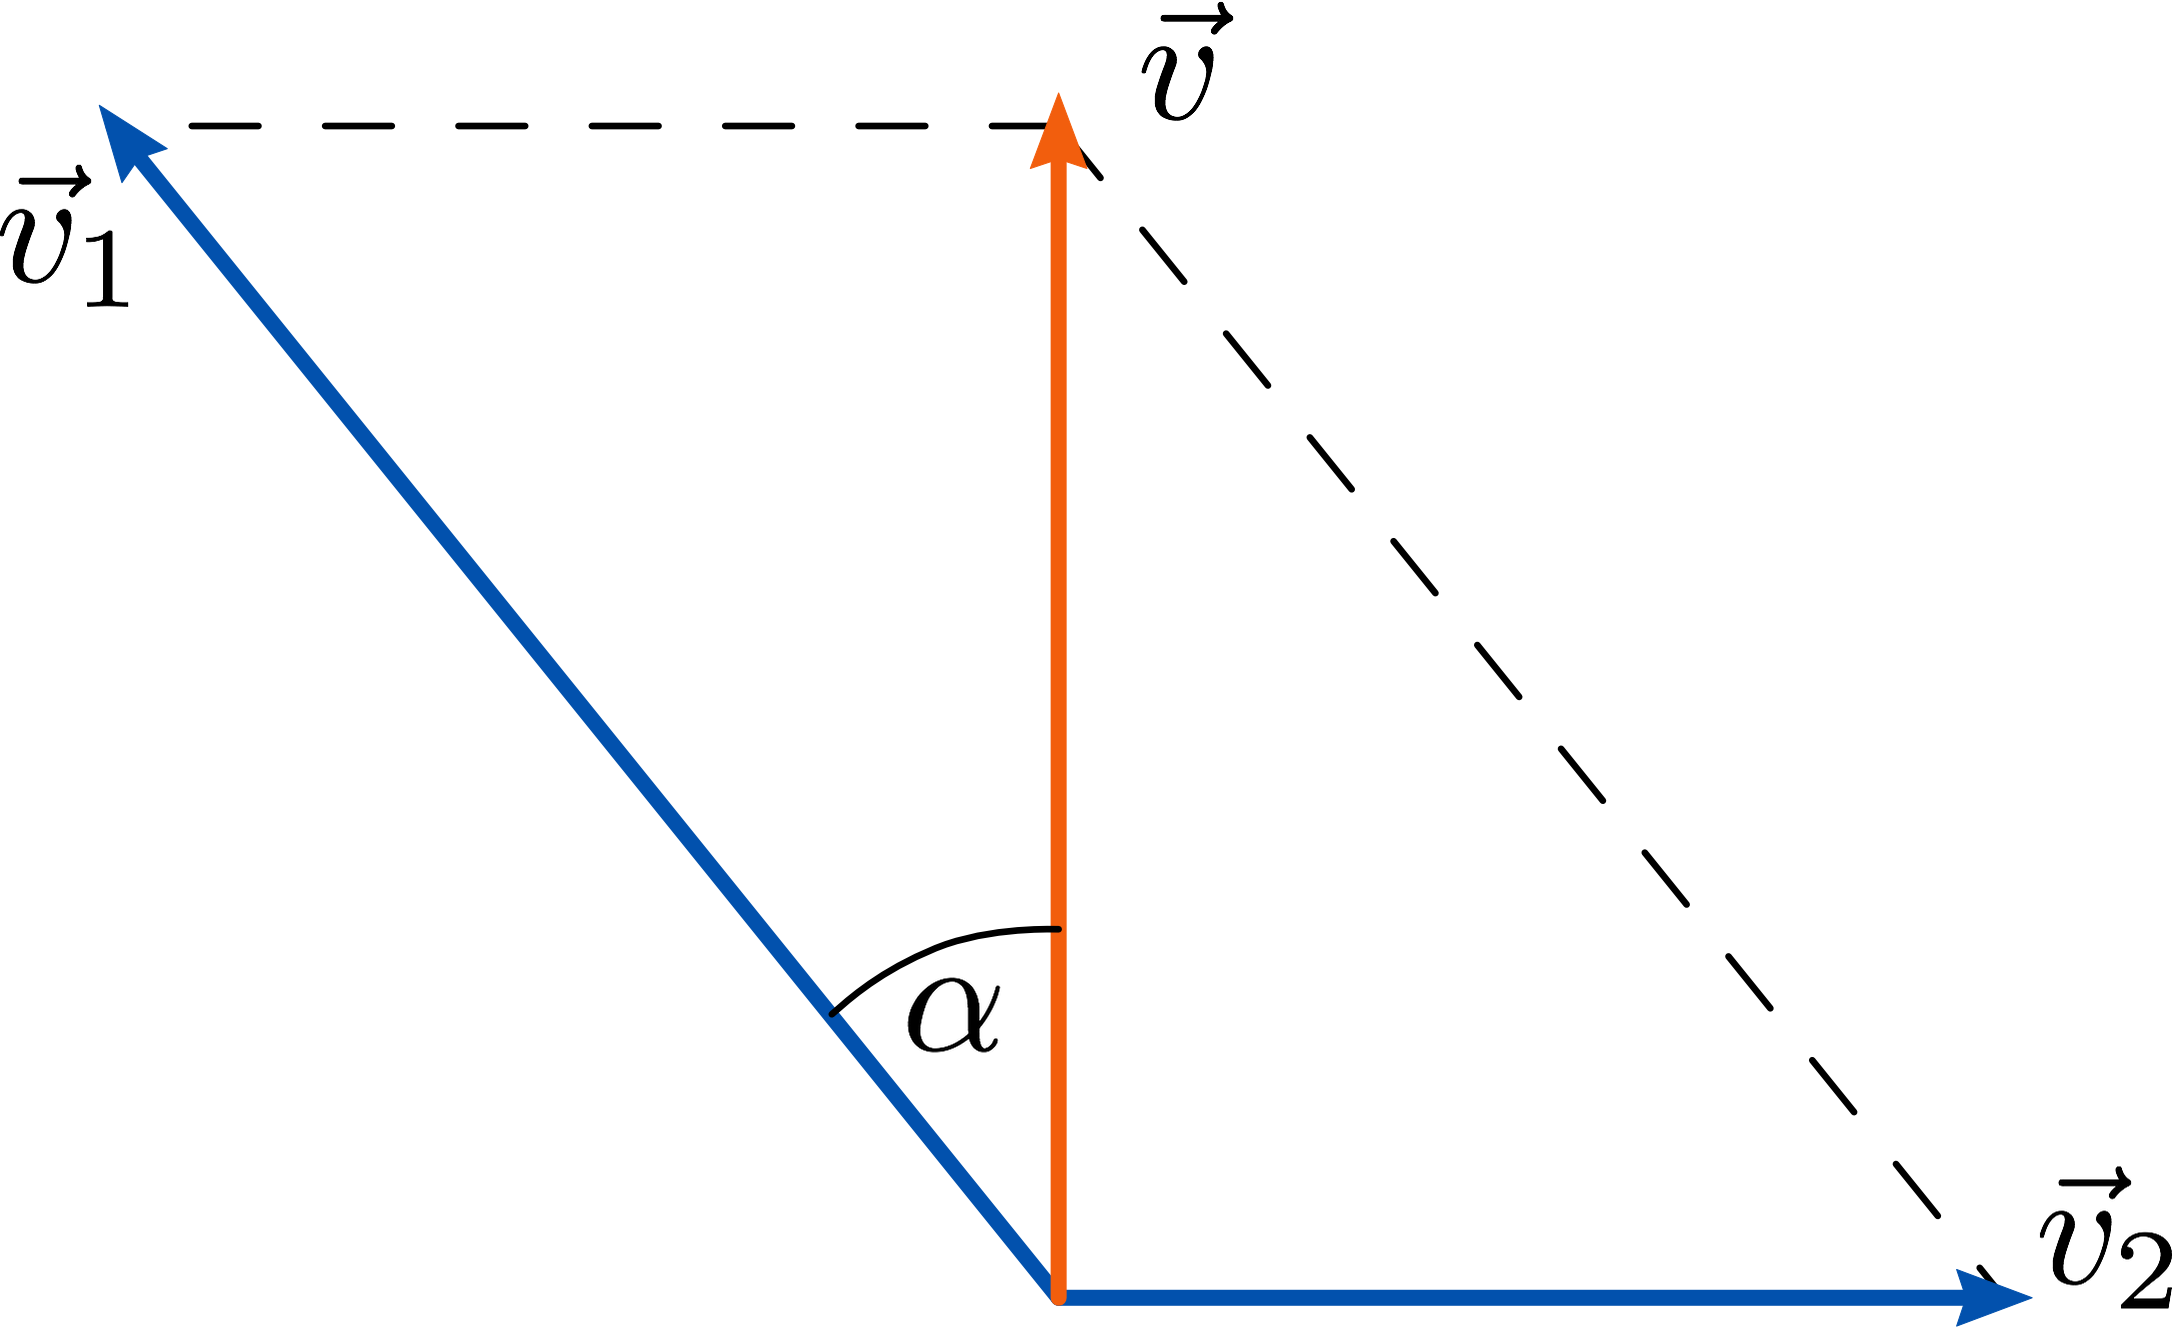
\includegraphics[width=\textwidth]{vectoren_veerman.png}
%    \end{column}
%\end{columns}
%\end{frame}
%
%%\begin{frame}{Oefening 16 p. 88}
%%\begin{figure}
%%\href{https://ophysics.com/k11.html}{%
%%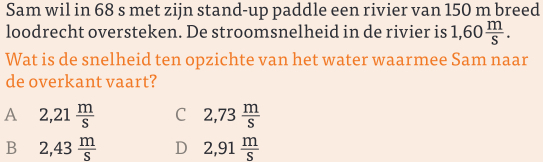
\includegraphics[width=\textwidth]{16p88}
%%}
%%\end{figure}
%%\end{frame}


\begin{frame}
	\frametitle{\href{https://www.geogebra.org/m/wvteqkrr}{Voorbeeldoefening}}
	\framesubtitle{}
	
	De plaatsvector van een deeltje wordt (voor $t\geq0$) gegeven door:
\begin{equation*}
	\vec{r}=-t\vec{e}_x+(t-1)^2\vec{e}_y
\end{equation*}

\begin{enumerate}

\item Geef de baanvergelijking.
\item Wanneer is \'e\'en van de snelheidscomponenten nul?
\item Hoe groot is dan de snelheid?
\item Waar is het deeltje dan?
\item Geef de versnellingsvector.
\item Raakt de versnellingsvector aan de baan? %Licht toe.

\end{enumerate}
	\hfill\href{run:./app/vb_2D.ggb}{\includegraphics[height=16pt]{electron-icon}}
\end{frame}

\note[itemize]{
\item $y(x)=(x+1)^2$
\item De snelheidscomponent volgens de $x$-as is nooit nul. Die volgens de $y$-as is nul wanneer: $2(t-1)=0$ oftewel wanneer $t=1$.
\item $v(1)=\sqrt{v_x^2+v_y^2}=\sqrt{(-1)^2+0^2}=\SI{1}{m/s}$
\item Nee, de versnellingsvector is niet rakend aan de baan. Hij is altijd verticaal ge\"ori\"enteerd terwijl de afgeleide van de baanvergelijking ($y'=2(x+1)$) overal bestaat en dus nergens een verticale helling heeft.
}




\usebackgroundtemplate{
\includegraphics[width=\paperwidth,height=\paperheight]{achtergrond22n}}